\documentclass{beamer}
\usepackage{amsmath}
\usepackage[english]{babel} %set language; note: after changing this, you need to delete all auxiliary files to recompile
\usepackage[utf8]{inputenc} %define file encoding; latin1 is the other often used option
\usepackage{csquotes} % provides context sensitive quotation facilities
\usepackage{graphicx} %allows for inserting figures
\usepackage{booktabs} % for table formatting without vertical lines
\usepackage{textcomp} % allow for example using the Euro sign with \texteuro
\usepackage{stackengine}
\usepackage{wasysym}
\usepackage{tikzsymbols}
\usepackage{textcomp}
\newcommand{\bubblethis}[2]{
        \tikz[remember picture,baseline]{\node[anchor=base,inner sep=0,outer sep=0]%
        (#1) {\underline{#1}};\node[overlay,cloud callout,callout relative pointer={(0.2cm,-0.7cm)},%
        aspect=2.5,fill=yellow!90] at ($(#1.north)+(-0.5cm,1.6cm)$) {#2};}%
    }%
\tikzset{face/.style={shape=circle,minimum size=4ex,shading=radial,outer sep=0pt,
        inner color=white!50!yellow,outer color= yellow!70!orange}}
%% Some commands to make the code easier
\newcommand{\emoticon}[1][]{%
  \node[face,#1] (emoticon) {};
  %% The eyes are fixed.
  \draw[fill=white] (-1ex,0ex) ..controls (-0.5ex,0.2ex)and(0.5ex,0.2ex)..
        (1ex,0.0ex) ..controls ( 1.5ex,1.5ex)and( 0.2ex,1.7ex)..
        (0ex,0.4ex) ..controls (-0.2ex,1.7ex)and(-1.5ex,1.5ex)..
        (-1ex,0ex)--cycle;}
\newcommand{\pupils}{
  %% standard pupils
  \fill[shift={(0.5ex,0.5ex)},rotate=80] 
       (0,0) ellipse (0.3ex and 0.15ex);
  \fill[shift={(-0.5ex,0.5ex)},rotate=100] 
       (0,0) ellipse (0.3ex and 0.15ex);}

\newcommand{\emoticonname}[1]{
  \node[below=1ex of emoticon,font=\footnotesize,
        minimum width=4cm]{#1};}
\usepackage{scalerel}
\usetikzlibrary{positioning}
\usepackage{xcolor,amssymb}
\newcommand\dangersignb[1][2ex]{%
  \scaleto{\stackengine{0.3pt}{\scalebox{1.1}[.9]{%
  \color{red}$\blacktriangle$}}{\tiny\bfseries !}{O}{c}{F}{F}{L}}{#1}%
}
\newcommand\dangersignw[1][2ex]{%
  \scaleto{\stackengine{0.3pt}{\scalebox{1.1}[.9]{%
  \color{red}$\blacktriangle$}}{\color{white}\tiny\bfseries !}{O}{c}{F}{F}{L}}{#1}%
}
\usepackage{fontawesome} % Social Icons
\usepackage{epstopdf} % allow embedding eps-figures
\usepackage{tikz} % allows drawing figures
\usepackage{amsmath,amssymb,amsthm} %advanced math facilities
\usepackage{lmodern} %uses font that support italic and bold at the same time
\usepackage{hyperref}
\usepackage{tikz}
\hypersetup{
    colorlinks=true,
    linkcolor=blue,
    filecolor=magenta,      
    urlcolor=blue,
}
\usepackage{tcolorbox}
%add citation management using BibLaTeX
\usepackage[citestyle=authoryear-comp, %define style for citations
    bibstyle=authoryear-comp, %define style for bibliography
    maxbibnames=10, %maximum number of authors displayed in bibliography
    minbibnames=1, %minimum number of authors displayed in bibliography
    maxcitenames=3, %maximum number of authors displayed in citations before using et al.
    minnames=1, %maximum number of authors displayed in citations before using et al.
    datezeros=false, % do not print dates with leading zeros
    date=long, %use long formats for dates
    isbn=false,% show no ISBNs in bibliography (applies only if not a mandatory field)
    url=false,% show no urls in bibliography (applies only if not a mandatory field)
    doi=false, % show no dois in bibliography (applies only if not a mandatory field)
    eprint=false, %show no eprint-field in bibliography (applies only if not a mandatory field)
    backend=biber %use biber as the backend; backend=bibtex is less powerful, but easier to install
    ]{biblatex}
\addbibresource{../mybibfile.bib} %define bib-file located one folder higher


\usefonttheme[onlymath]{serif} %set math font to serif ones

\definecolor{beamerblue}{rgb}{0.2,0.2,0.7} %define beamerblue color for later use

%%% defines highlight command to set text blue
\newcommand{\highlight}[1]{{\color{blue}{#1}}}


%%%%%%% commands defining backup slides so that frame numbering is correct

\newcommand{\backupbegin}{
   \newcounter{framenumberappendix}
   \setcounter{framenumberappendix}{\value{framenumber}}
}
\newcommand{\backupend}{
   \addtocounter{framenumberappendix}{-\value{framenumber}}
   \addtocounter{framenumber}{\value{framenumberappendix}}
}

%%%% end of defining backup slides

%Specify figure caption, see also http://tex.stackexchange.com/questions/155738/caption-package-not-working-with-beamer
\setbeamertemplate{caption}{\insertcaption} %redefines caption to remove label "Figure".
%\setbeamerfont{caption}{size=\scriptsize,shape=\itshape,series=\bfseries} %sets figure  caption bold and italic and makes it smaller


\usetheme{Boadilla}

%set options of hyperref package
\hypersetup{
    bookmarksnumbered=true, %put section numbers in bookmarks
    naturalnames=true, %use LATEX-computed names for links
    citebordercolor={1 1 1}, %color of border around cites, here: white, i.e. invisible
    linkbordercolor={1 1 1}, %color of border around links, here: white, i.e. invisible
    colorlinks=true, %color links
    anchorcolor=black, %set color of anchors
    linkcolor=beamerblue, %set link color to beamer blue
    citecolor=blue, %set cite color to beamer blue
    pdfpagemode=UseThumbs, %set default mode of PDF display
    breaklinks=true, %break long links
    pdfstartpage=1 %start at first page
    }


% --------------------
% Overall information
% --------------------
\title[Principios de Economía]{Principios de Economía}
\date{}
\author[Ertola y Sturzenegger]{Gabriela Ertola y Federico Sturzenegger }
\vspace{0.4cm}
\institute[]{Universidad de San Andrés \\
2022} 


\begin{document}

\begin{frame}
\frametitle{Principios de Economía
\centering
\\ \vspace{12mm} Distorciones}
\centering
 \\ \vspace{12mm} %5 de agosto, 2021 \vspace{5mm} \\ 

\includegraphics[scale=0.25]{Figures/logoUDESA.jpg} 
\end{frame}


\begin{frame}{Mercados vs Planificación}
    
    \begin{itemize}
        \item ¿Cuál era el problema económico?
        \item ¿Se acuerdan el ejemplo de los tazones? 
        \vspace{1mm}
        \item El ejemplo nos permite ilustrar los problemas de la asignación considerando distintos mecanismos: asignación de mercado versus planificación
        \vspace{1mm}
        \item ¡Y también comparar estos mecanismos! 
    \end{itemize}
\end{frame}

\begin{frame}{Algunos problemas de la planificación}
    \begin{itemize}
        \item Es muy intensivo en información requerida (necesita conocer perfectamente preferencias y costos)  \vspace{1mm}
            \begin{itemize} [l{-}] 
                \item  Ejemplo de Cheqoslovaquia
            \end{itemize}
            \vspace{1mm}
        \item Genera incentivos incorrectos  \vspace{1mm}
            \begin{itemize} [l{-}]
                \item Ejemplo de la China Maoísta
            \end{itemize}
            \vspace{1mm}
        \item Resulta inconsistente con las libertades políticas  ''
            \begin{itemize} [l{-}]
                \item ``El camino a la servidumbre'' de Hayek     
            \end{itemize}
            \begin{itemize} [l{-}]
                \item Concepto de ``Libertad como desarrollo'' de Amartya Sen
            \end{itemize}
    \end{itemize}
\end{frame}

\begin{frame}{La peli recomendada}
    \centering  
    \href{https://www.youtube.com/watch?v=u5hzmwGW4Ac}{
\includegraphics[scale=0.95]{Figures/Goodbyelenin.png}}  
\end{frame}

\begin{frame}{La mano invisible de Adam Smith}
    \begin{quote}
    “No es la benevolencia del carnicero, cervecero o panadero de donde obtendremos nuestra cena, sino de su preocupación por sus propios intereses”
\end{quote}
\end{frame}

\begin{frame}{Eficiencia de mercado}

     \begin{figure}[H]{\textwidth}
         \centering
         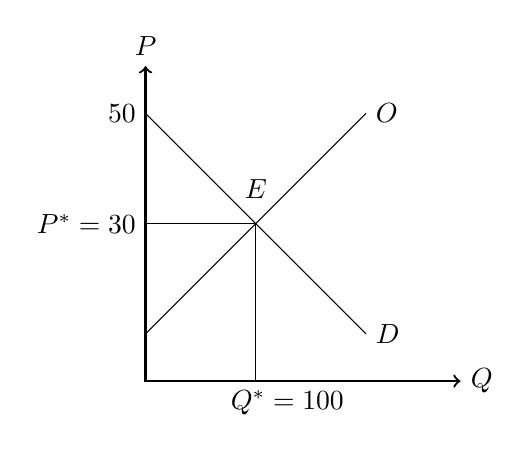
\begin{tikzpicture}[scale=0.4]
\draw[thick,<->] (0,10) node[above]{$P$}--(0,0)--(10,0) node[right]{$Q$};
%\node [below left] at (0,0) {$0$};
\node [below] at (4.5,0) {$Q^*=100$};
\node [above] at (7/2,5.5) {$E$};
\node [left] at (0,5) {$P^*=30$};
%\node [left] at (0,6.85) {$40$};
\node [left] at (0,8.5) {$50$};
%\node [below] at (1.75,0) {50};
%\draw[semithick, red](1.75,5)--(1.75,6.85);
%\draw[thick,gray, dashed](1.75,0)--(1.75,6.85)--(0,6.85);
\draw[](0,5)--(7/2,5)--(7/2,0);
\draw[black, domain=0:7] plot (\x, {8.5-\x}) node[right] {$D$};
\draw[black, domain=0:7] plot (\x, {1.5+\x}) node[right] {$O$};
\end{tikzpicture}
     \end{figure}
El mercado produce la cantidad óptima del bien: solo se produce si vale más que lo que cuesta producirlo
\end{frame}

\begin{frame}{Eficiencia de mercado II}

    \begin{figure}{\textwidth}
         \centering
         \tikzset{every picture/.style={line width=0.75pt}} %set default line width to 0.75pt        
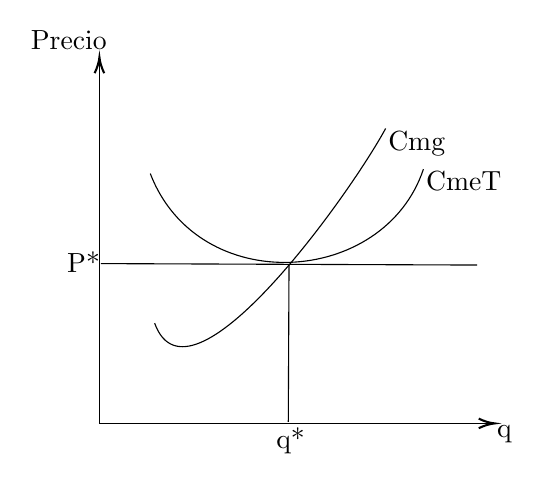
\begin{tikzpicture}[x=0.75pt,y=0.75pt,yscale=-0.7,xscale=0.7] 
%uncomment if require: \path (0,1657); %set diagram left start at 0, and has height of 1657

%Straight Lines [id:da6123979361342768] 
\draw    (74,298) -- (344,298) ;
\draw [shift={(346,298)}, rotate = 180] [color={rgb, 255:red, 0; green, 0; blue, 0 }  ][line width=0.75]    (10.93,-3.29) .. controls (6.95,-1.4) and (3.31,-0.3) .. (0,0) .. controls (3.31,0.3) and (6.95,1.4) .. (10.93,3.29)   ;
%Straight Lines [id:da5131707791527922] 
\draw    (74,298) -- (74,48) ;
\draw [shift={(74,46)}, rotate = 450] [color={rgb, 255:red, 0; green, 0; blue, 0 }  ][line width=0.75]    (10.93,-3.29) .. controls (6.95,-1.4) and (3.31,-0.3) .. (0,0) .. controls (3.31,0.3) and (6.95,1.4) .. (10.93,3.29)   ;
%Straight Lines [id:da6346804843028921] 
\draw    (75,188) -- (334,189) ;
%Curve Lines [id:da697350144213293] 
\draw    (109,126) .. controls (142,212) and (270,204) .. (297,123) ;
%Curve Lines [id:da9799910224345574] 
\draw    (112,229) .. controls (136,295) and (246,141) .. (271,95) ;
%Straight Lines [id:da5845279516726063] 
\draw    (204.5,188.5) -- (204,297) ;

% Text Node
\draw (25,26) node [anchor=north west][inner sep=0.75pt]   [align=left] {Precio};
% Text Node
\draw (346,298) node [anchor=north west][inner sep=0.75pt]   [align=left] {q};
% Text Node
\draw (297,123) node [anchor=north west][inner sep=0.75pt]   [align=left] {CmeT};
% Text Node
\draw (271,95) node [anchor=north west][inner sep=0.75pt]   [align=left] {Cmg};
% Text Node
\draw (50,178) node [anchor=north west][inner sep=0.75pt]   [align=left] {P*};
% Text Node
\draw (194,299) node [anchor=north west][inner sep=0.75pt]   [align=left] {q*};

\end{tikzpicture}
     \end{figure}

En el largo plazo, el mercado produce cada bien al MENOR costo medio posible dada la tecnología
\end{frame}

\begin{frame}{Distorsiones al equilibrio de mercado}
    \begin{itemize}
        \item En muchas ocasiones el mercado no funciona tan perfectamente
        \vspace{1mm}
        \item Hay dos tipos de desvíos
        \begin{itemize}
            \item Los creados por el hombre
            \item Los que se imponen por características de la realidad
        \end{itemize}
    \end{itemize}
\end{frame}


\begin{frame}{Distorsiones al equilibrio de mercado}
    \begin{itemize}
        \item Creadas por el hombre:
        \begin{itemize}
            \item Monopolios artificiales (farmacias, escribanos, low cost)
             \vspace{1mm}
            \item Impuestos
             \vspace{1mm}
            \item Precios máximos o mínimos (cepo)
             \vspace{1mm}
            \item Regulación (ley de alquileres)
        \end{itemize}
    \end{itemize}
\end{frame}

\begin{frame}{Distorsiones al equilibrio de mercado}
    \begin{itemize}
        \item Por las características de la realidad \vspace{1mm}
        \begin{itemize}
            \item Monopolios naturales (red eléctrica, agua, gas)   
             \vspace{1mm}
            \item Externalidades
             \vspace{1mm}
            \item Bienes públicos
            \vspace{1mm}
            \item Problemas de información
            \begin{itemize}
                \item Atributos ocultos (selección adversa)
                 \vspace{1mm}
                \item Acciones ocultas (moral hazard)
            \end{itemize}        
        \end{itemize}
    \end{itemize}
\end{frame}

\begin{frame}{La introducción de un impuesto}

\begin{figure} [H]
\caption{¡Genera un costo de eficiencia!}
   \centering
\begin{tikzpicture}[scale=0.6]
\draw[very thick,<->] (0,10) node[above]{$P$}--(0,0)--(10,0) node[right]{$Q$};
\draw[semithick](1,2)--(8,9) node[right]{$O'$};
\draw[semithick](2,1)--(9,8) node[right]{$O$};
\draw[semithick](1,9)--(9,1) node[right]{$D$};
\path[pattern=horizontal lines,pattern color=black] (4.5,3.6)--(4.5,5.5)--(5.4,4.5);
\draw[semithick,dashed,gray](0,5.5)--(4.5,5.5)--(4.5,0);
\draw[semithick,dashed, gray](0,3.6)--(4.5,3.6);
\node [right] at (7,5) {\scriptsize Triángulo de};
\node [right] at (7.25,4.5) {\scriptsize Harberger};
\draw[semithick, <-] (5.3,4.2)..controls (5.8,3.8) and (6.8,3.8)..(7.5,4.2);
\draw[semithick,dashed,gray](0,4.5)--(5.5,4.5)--(5.5,0);
\node[below] at(5.5,0) {\footnotesize $Q*$};
\node[below] at(4.5,0) {\footnotesize $Q'$};
\node[left] at(0,4.5) {\footnotesize $P*$};
\node[left] at(0,5.5) {\footnotesize $P'_C$};
\node[left] at(0,3.6) {\footnotesize $P'_P$};
\end{tikzpicture}
\label{fig:20.2}
\end{figure}

\end{frame}

\begin{frame}{Minimizando las distorsiones}

\begin{figure} [H]
\caption{Impuestos con producto totalmente inelástico}
    \centering
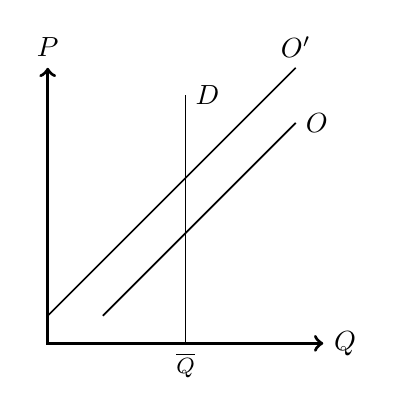
\begin{tikzpicture}[scale=0.35]
\draw[ very thick,<->] (0,10) node[above]{$P$}--(0,0)--(10,0) node[right]{$Q$};
%\node [below left] at (0,0) {$0$};
\draw[semithick](0,1)--(9,10) node[above]{$O'$};
\draw[semithick](2,1)--(9,8) node[right]{$O$};
\draw[semithick](5,0)--(5,9) node[right]{$D$};
\node[below] at(5,0) {\footnotesize $\overline{Q}$};
\end{tikzpicture}
\label{fig:20.1}
\end{figure} 

\begin{itemize}
    \item Queremos grabar los bienes más inelásticos
    \item Si todos los bienes tienen la misma elasticidad entonces tendran la misma tasa
\end{itemize}
\end{frame}

\begin{frame}{Incidencia de los impuestos}
\begin{figure} [H]
\caption{Veamos en quién recae el impuesto...}
   \centering
\begin{tikzpicture}[scale=0.6]
\draw[very thick,<->] (0,10) node[above]{$P$}--(0,0)--(10,0) node[right]{$Q$};
\draw[semithick](1,2)--(8,9) node[right]{$O'$};
\draw[semithick](2,1)--(9,8) node[right]{$O$};
\draw[semithick](1,9)--(9,1) node[right]{$D$};
\path[pattern=horizontal lines,pattern color=black] (4.5,3.55)--(4.5,5.5)--(5.4,4.5);
\path[pattern=north lines,pattern color=black] (0,4.5)--(3.55,5.5);
\draw[semithick,dashed,gray](0,5.5)--(4.5,5.5)--(4.5,0);
\draw[semithick,dashed, gray](0,3.6)--(4.5,3.55);
\node [right] at (7,5) {\scriptsize Triángulo de};
\node [right] at (7.25,4.5) {\scriptsize Harberger};
\draw[semithick, <-] (5.3,4.2)..controls (5.8,3.8) and (6.8,3.8)..(7.5,4.2);
\draw[semithick,dashed,gray](0,4.5)--(5.5,4.5)--(5.5,0);
\draw [pattern=north west lines, pattern color=red] (0,4.5) rectangle (4.5,5.5);
\draw [pattern=north west lines, pattern color=blue] (0,3.55) rectangle (4.5,4.5);
\node[below] at(5.5,0) {\footnotesize $Q*$};
\node[below] at(4.5,0) {\footnotesize $Q'$};
\node[left] at(0,4.5) {\footnotesize $P*$};
\node[left] at(0,5.5) {\footnotesize $P'_C$};
\node[left] at(0,3.55) {\footnotesize $P'_P$};
\end{tikzpicture}
\label{fig:20.2}
\end{figure}
\end{frame}


\begin{frame}{Precios Máximos}
\begin{figure} [H]
\caption{Precio Máximo}
    \centering
\begin{tikzpicture}[scale=0.6]
\draw[very thick,<->] (0,10) node[above]{$P$}--(0,0)--(10,0) node[right]{$Q$};
\draw[semithick](1,1)--(9,9) node[right]{$O$};
\draw [semithick] (1,9)--(9,1) node[right]{$D$};
\draw [pattern=north west lines, pattern color=blue] (0,3) rectangle (3,7);
\draw[thick, gray, dashed](3,0)--(3,7) ;
\draw[semithick, gray](0,3)--(7,3);
\draw[thick, gray, dashed](5,0)--(5,5) ;
\draw[thick, gray, dashed](0,5)--(5,5) ;
\draw[thick, gray, dashed](7,0)--(7,3) ;
\draw[semithick, gray](0,7)--(3,7);
%\draw[semithick, gray,dashed](3,3)--(7.5,3);
\node[left] at (0,3){\footnotesize $P_{max}$};
\node[left] at (0,7){\footnotesize $P_{ilegal}$};
\node[left] at (0,5){\footnotesize $P*$};
\node[below] at (5,0){\footnotesize $Q*$};
\node[below] at (3,0){\footnotesize $Q_{P_{max}}^{O}$};
\node[below] at (7,0){\footnotesize $Q_{P_{max}}^{D}$};
\draw[semithick, <-] (1.75,7.15).. controls (2.25,8) and (2.75,8).. (3.5,7.75);
\node[above] at (5,7.5) {\tiny Margen};
\node[above] at (5,7.25) {\tiny Intermediarios};
\end{tikzpicture}
\label{fig:20.6}
\end{figure}  
\end{frame}

\begin{frame}{ Precios sostén}
\begin{figure} [H]
\centering
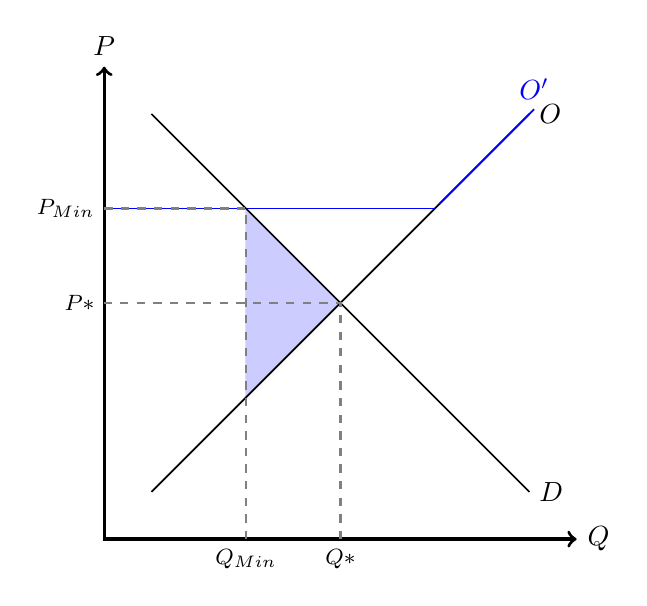
\begin{tikzpicture}[scale=0.6]
\draw[very thick,<->] (0,10) node[above]{$P$}--(0,0)--(10,0) node[right]{$Q$};
\draw[fill,blue!20] (5,5)--(3,7)--(3,3);
\draw [semithick](1,1)--(9,9) node[right]{$O$};
\draw [semithick, blue](7.1,7.1)--(9.1,9.1) node[above]{$O'$};
\draw [semithick, blue](7,7)--(0,7);
\draw [semithick](1,9)--(9,1) node[right]{$D$};
\draw[thick, gray, dashed](3,0)--(3,7) ;
\draw[thick, gray, dashed](0,7)--(3,7) ;
\draw[thick, gray, dashed](5,0)--(5,5)--(0,5) ;
%\node[left] at (0,3){\footnotesize $P^{'}_D$};
\node[left] at (0,7){\footnotesize $P_{Min}$};
\node[below] at (3,0){\footnotesize $Q_{Min}$};
\node[left] at (0,5){\footnotesize $P*$};
\node[below] at (5,0){\footnotesize $Q*$};
\end{tikzpicture}
\label{fig:20.7}
\end{figure} 
\end{frame}

\begin{frame}{Precios sostén con mercado paralelo}
\begin{figure} [H]
\centering
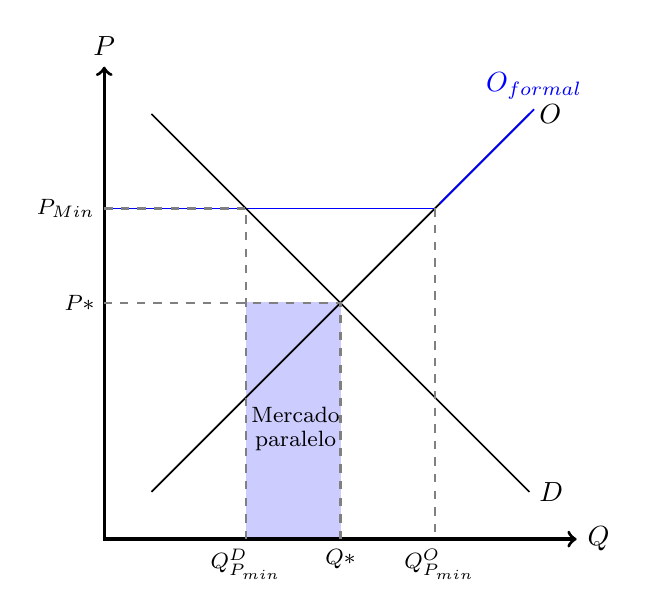
\begin{tikzpicture}[scale=0.6]
\draw[very thick,<->] (0,10) node[above]{$P$}--(0,0)--(10,0) node[right]{$Q$};
\draw[fill,blue!20] (3,0.05)--(5,0.05)--(5,5)--(3,5);
\draw [semithick](1,1)--(9,9) node[right]{$O$};
\draw [semithick, blue](7.1,7.1)--(9.1,9.1) node[above]{$O_{formal}$};
\draw [semithick, blue](7,7)--(0,7);
\draw [semithick](1,9)--(9,1) node[right]{$D$};
\draw[thick, gray, dashed](3,0)--(3,7) ;
\draw[thick, gray, dashed](0,7)--(3,7) ;
%\draw[thick, gray, dashed](0,7)--(7,7)--(7,3)--(0,3) ;
\draw[thick, gray, dashed](5,0)--(5,5)--(0,5) ;
\draw[thick, gray, dashed](7,7)--(7,0) ;
%\node[left] at (0,3){\footnotesize $P^{'}_D$};
\node[left] at (0,7){\footnotesize $P_{Min}$};
\node[below] at (3,0){\footnotesize $Q_{P_{min}}^{D}$};
\node[below] at (7.1,0){\footnotesize $Q_{P_{min}}^{O}$};
\node[left] at (0,5){\footnotesize $P*$};
\node[below] at (5,0){\footnotesize $Q*$};
\node[below] at (4.05,3){\footnotesize Mercado};
\node[below] at (4.05,2.5){\footnotesize paralelo};
\end{tikzpicture}
\label{fig:20.7b}
\end{figure}  
\end{frame}

\begin{frame}{Precios sostén con adquisición del excedente}
\begin{figure} [H]
\caption{Sin reventa}
\centering
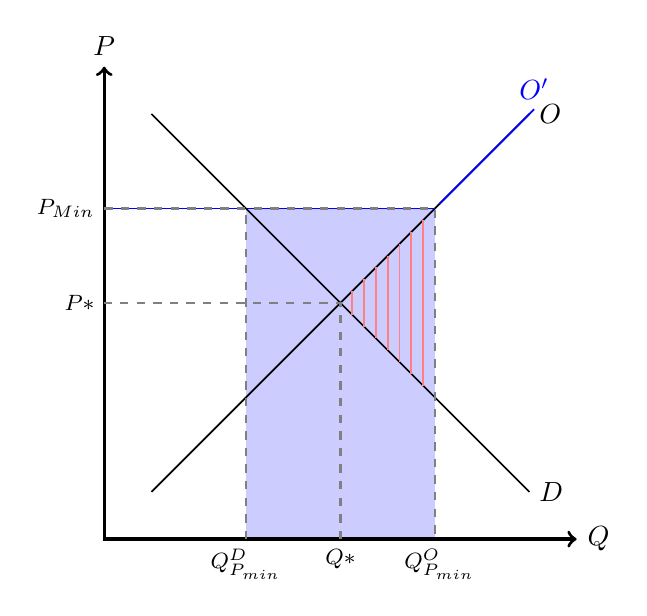
\begin{tikzpicture}[scale=0.6]
\draw[very thick,<->] (0,10) node[above]{$P$}--(0,0)--(10,0) node[right]{$Q$};
\draw[fill,blue!20] (3,0.05)--(7,0.05)--(7,7)--(3,7);
\draw [semithick](1,1)--(9,9) node[right]{$O$};
\draw [semithick, blue](7.1,7.1)--(9.1,9.1) node[above]{$O'$};
\draw [semithick, blue](7,7)--(0,7);
\draw [semithick](1,9)--(9,1) node[right]{$D$};
\draw[semithick, red!50] (6.75,3.25)--(6.75,6.75);
\draw[semithick, red!50] (6.5,3.5)--(6.5,6.5);
\draw[semithick, red!50] (6.25,3.75)--(6.25,6.25);
\draw[semithick, red!50] (6,4)--(6,6);
\draw[semithick, red!50] (5.75,4.25)--(5.75,5.75);
\draw[semithick, red!50] (5.5,4.5)--(5.5,5.5);
\draw[semithick, red!50] (5.25,4.75)--(5.25,5.25);
%\draw[thick, gray, dashed](2,0)--(2,7) ;
\draw[thick, gray, dashed](0,7)--(2,7) ;
\draw[thick, gray, dashed](0,7)--(7,7)--(7,0) ;
\draw[thick, gray, dashed](5,0)--(5,5)--(0,5) ;
\draw[thick, gray, dashed](3,0)--(3,7);
\node[left] at (0,7){\footnotesize $P_{Min}$};
\node[below] at (3,0){\footnotesize $Q_{P_{min}}^{D}$};
\node[below] at (7.1,0){\footnotesize $Q_{P_{min}}^{O}$};
\node[left] at (0,5){\footnotesize $P*$};
\node[below] at (5,0){\footnotesize $Q*$};
\end{tikzpicture}
\label{fig:20.7c}
\end{figure} 

\end{frame}

\begin{frame}{Precios sostén con adquisición del excedente}
\begin{figure} [H]
\caption{Con reventa}
\centering
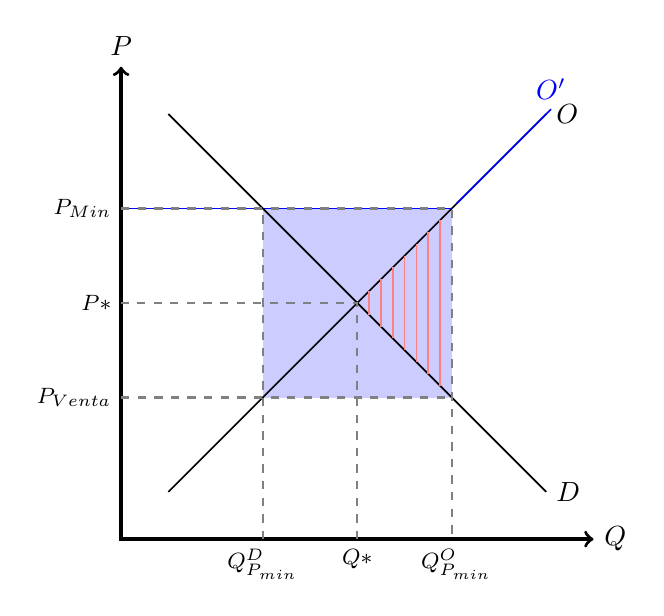
\begin{tikzpicture}[scale=0.6]
\draw[very thick,<->] (0,10) node[above]{$P$}--(0,0)--(10,0) node[right]{$Q$};
\draw[fill,blue!20] (3,3)--(7,3)--(7,7)--(3,7);
\draw [semithick](1,1)--(9,9) node[right]{$O$};
\draw [semithick, blue](7.1,7.1)--(9.1,9.1) node[above]{$O'$};
\draw [semithick, blue](7,7)--(0,7);
\draw [semithick](1,9)--(9,1) node[right]{$D$};
\draw[semithick, red!50] (6.75,3.25)--(6.75,6.75);
\draw[semithick, red!50] (6.5,3.5)--(6.5,6.5);
\draw[semithick, red!50] (6.25,3.75)--(6.25,6.25);
\draw[semithick, red!50] (6,4)--(6,6);
\draw[semithick, red!50] (5.75,4.25)--(5.75,5.75);
\draw[semithick, red!50] (5.5,4.5)--(5.5,5.5);
\draw[semithick, red!50] (5.25,4.75)--(5.25,5.25);
%\draw[thick, gray, dashed](2,0)--(2,7) ;
\draw[thick, gray, dashed](0,7)--(2,7) ;
\draw[thick, gray, dashed](0,7)--(7,7)--(7,0) ;
\draw[thick, gray, dashed](5,0)--(5,5)--(0,5) ;
\draw[thick, gray, dashed](3,0)--(3,7) ;
\draw[thick, gray, dashed](0,3)--(7,3) ;
%\node[left] at (0,3){\footnotesize $P^{'}_D$};
\node[left] at (0,7){\footnotesize $P_{Min}$};
\node[left] at (0,3){\footnotesize $P_{Venta}$};
\node[below] at (3,0){\footnotesize $Q_{P_{min}}^{D}$};
\node[below] at (7.1,0){\footnotesize $Q_{P_{min}}^{O}$};
\node[left] at (0,5){\footnotesize $P*$};
\node[below] at (5,0){\footnotesize $Q*$};
\end{tikzpicture}
\label{fig:20.7c}
\end{figure} 
\end{frame}

%\begin{frame}{15. El mercado de Berlín}
%    \begin{figure}[htp]
%\href{https://twitter.com/andreaskluth/status/1366691926804754440} {\makebox[\textwidth][c]{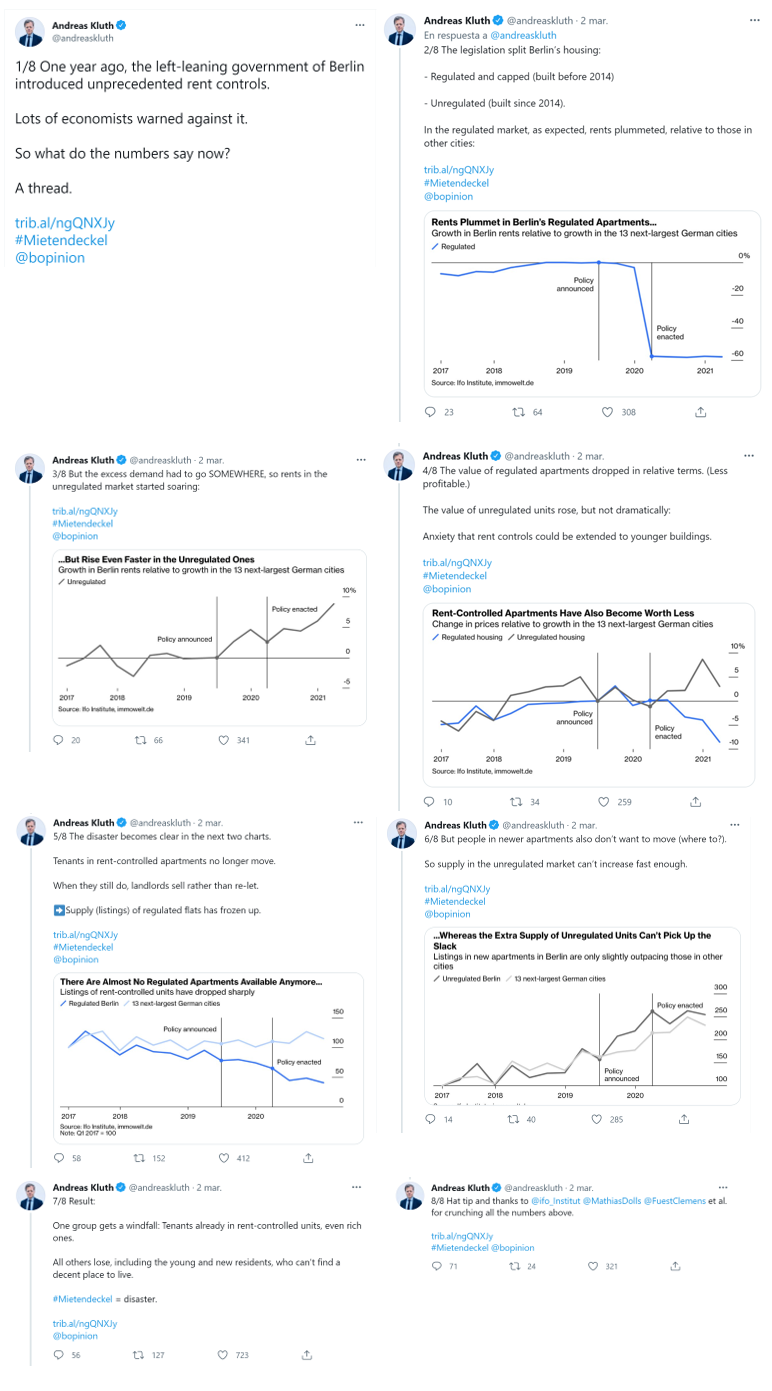
\includegraphics[width=0.45\textwidth]{images/TW.1.png}}} 
%\end{figure}
%Son muchos tweet en un imagen y para que entre todo queda muy chico. Igual haciendo click te lleva al hilo.
%\end{frame}

\begin{frame}{ Distorsiones del Monopolio}
\begin{figure} [H]
\centering
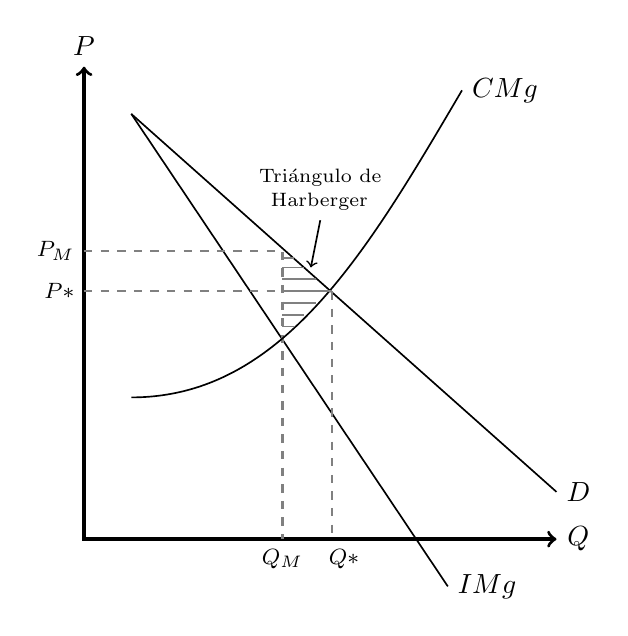
\begin{tikzpicture}[scale=0.6]
\draw[very thick,<->] (0,10) node[above]{$P$}--(0,0)--(10,0) node[right]{$Q$};
\draw[semithick](1,9)--(10,1) node[right]{$D$};
\draw[semithick](1,9)--(7.7,-1) node[right]{$IMg$};
\draw[thick,dashed,gray](0,6.1)--(4.2,6.1)--(4.2,0);
\draw[thick,dashed,gray](0,5.25)--(5.25,5.25)--(5.25,0);
%\draw(1,1)--(9,9);
\draw[semithick](1,3).. controls (4.2,3) and (6,6.1)..(8,9.5) node[right]{$CMg$};
\draw[semithick, gray] (4.2,5.95) to (4.45,5.95) ;
\draw[semithick, gray] (4.2,5.75) to (4.65,5.75) ;
\draw[semithick, gray] (4.2,5.5) to (4.9,5.5) ;
\draw[semithick, gray] (4.2,5.25) to (5.25,5.25) ;
\draw[semithick, gray] (4.2,5) to (4.9,5) ;
\draw[semithick, gray] (4.2,4.75) to (4.65,4.75) ;
\draw[semithick, gray] (4.2,4.5) to (4.45,4.5) ;
 \node [right] at (3.5,7.65) {\scriptsize Triángulo de};
 \node [right] at (3.75,7.15) {\scriptsize Harberger};
\draw[semithick, <-] (4.8,5.75)--(5,6.75);
\node[below] at(4.2,0) {\footnotesize $Q_M$};
\node[below] at(5.5,0) {\footnotesize $Q*$};
\node[left] at(0,6.1) {\footnotesize $P_{M}$};
\node[left] at(0,5.25) {\footnotesize $P*$};
\end{tikzpicture}
\label{fig:20.4}
\end{figure}
\end{frame}

  \begin{frame}{¿Eliminar al monopolio?}
    \begin{itemize}
        \item Lo primero que hay que hacer es entender porque hay un monopolio
        \item Y tratar de eliminarlo
        \item ¿Alcanza con decir que una empresa es grande para definir un monopolio? 
        \item No! ... si los mercados son contestables
        \item Solo en casos extremos debiéramos apelar a la regulación de precios
    \end{itemize}
\end{frame}

\begin{frame}{¿Cómo podemos regular un monopolio?}
\begin{figure} [H]
\caption{Precio Máximo en P*}
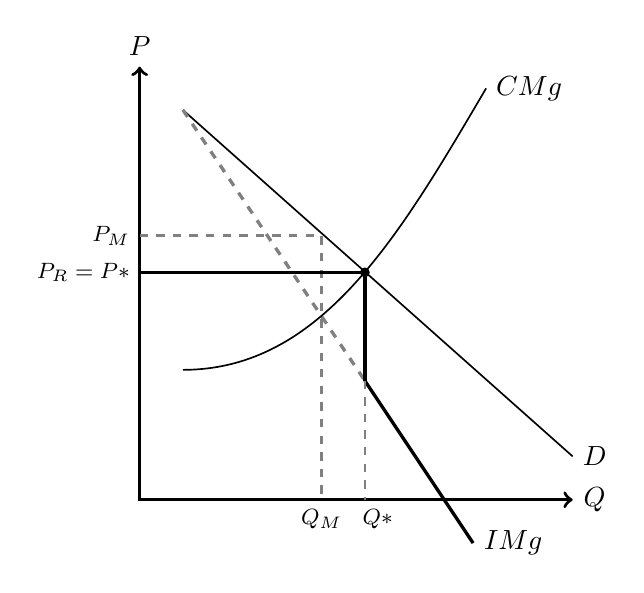
\begin{tikzpicture}[scale=0.55]
\draw[very thick,<->] (0,10) node[above]{$P$}--(0,0)--(10,0) node[right]{$Q$};
\draw[semithick](1,9)--(10,1) node[right]{$D$};
%\draw[semithick](1,9)--(7.7,-1) node[right]{$IMg$};
\draw[very thick,dashed,gray](1,9)--(5.2,2.75);
\draw[very thick](5.2,2.75)--(7.7,-1) node[right]{$IMg$};
\draw[thick,dashed,gray](5.2,2.75)--(5.2,0);
\draw[thick,dashed,gray](0,6.1)--(4.2,6.1)--(4.2,0);
\draw[very thick](0,5.25)--(5.2,5.25)--(5.2,2.75);
%\draw(1,1)--(9,9);
\draw[semithick](1,3).. controls (4.2,3) and (6,6.1)..(8,9.5) node[right]{$CMg$};
\node[below] at(4.2,0) {\footnotesize $Q_M$};
\node[below] at(5.5,0) {\footnotesize $Q*$};
\node[left] at(0,6.1) {\footnotesize $P_{M}$};
\node[left] at(0,5.25) {\footnotesize $P_{R}=P*$};
\draw[fill](5.2,5.25) circle [radius =0.1];
    \end{tikzpicture}
\label{fig:20.5}
\end{figure} 

\end{frame}


\begin{frame}{ Monopolio Natural}
\begin{figure} [H]
\centering
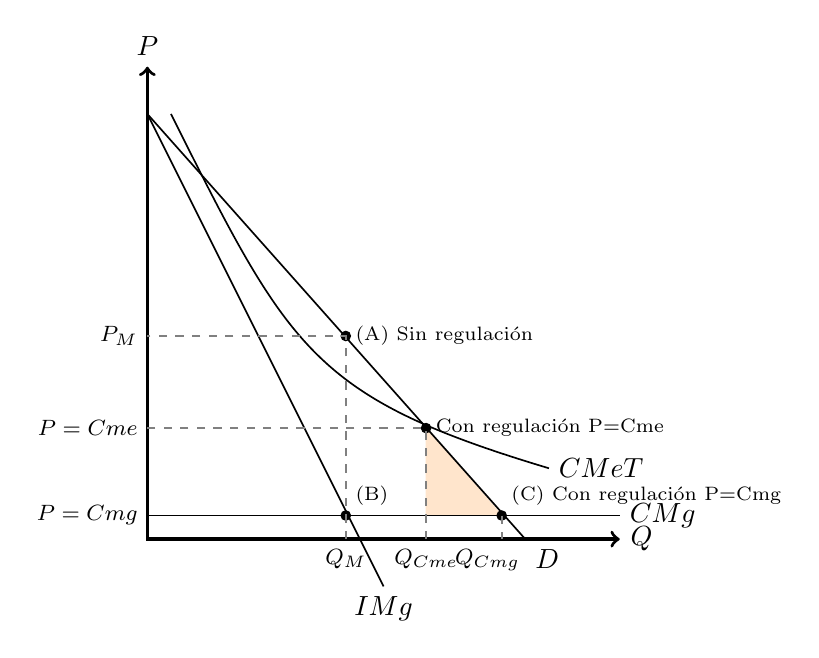
\begin{tikzpicture}[scale=0.6]
\draw[very thick,<->] (0,10) node[above]{$P$}--(0,0)--(10,0) node[right]{$Q$};
\draw[fill,orange!20]
(5.9,0.5)--(5.9,2.35)--(7.5,0.5);


\node[left] at (0,4.3) {\footnotesize $P_M$};
\node[below] at (4.2,0) {\footnotesize $Q_M$};
\node[left] at (0,2.35) {\footnotesize $P={Cme}$};
\node[below] at (5.9,0) {\footnotesize $Q_{Cme}$};
\node[left] at (0,0.5) {\footnotesize $P={Cmg}$};
\node[below] at (7.2,0) {\footnotesize $Q_{Cmg}$};


\draw[fill] (4.2,4.3) circle [radius =0.1] node[right] {\scriptsize (A) Sin regulación};
\draw[fill] (5.9,2.35) circle [radius =0.1] node[right] {\scriptsize Con regulación P=Cme};
\draw[fill] (7.5,0.5) circle [radius =0.1] node[above right] {\scriptsize (C) Con regulación P=Cmg};
\draw[fill] (4.2,0.5) circle [radius =0.1] node[above right] {\scriptsize (B)};


\draw[semithick](0,9)--(8,0) node[below right]{$D$};
\draw[semithick](0,9)--(5,-1) node[below]{$IMg$};
\draw[semithick](0,0.5)--(10,0.5) node[right]{$CMg$};
\draw[semithick](0.5,9) ..controls (3,4) and (3.5,3) .. (8.5,1.5) node[right]{$CMeT$};

\draw[thick, dashed,gray] (4.2,0)--(4.2,4.3)--(0,4.3);
\draw[thick, dashed,gray] (5.9,0)--(5.9,2.35)--(0,2.35);
\draw[thick, dashed,gray] (7.5,0.5)--(7.5,0);

\end{tikzpicture}
\label{fig:MNN}
\end{figure} 
\end{frame}


\begin{frame}{Poniéndole precio a una carretera  I}
     \begin{figure} [h!]
    \centering
    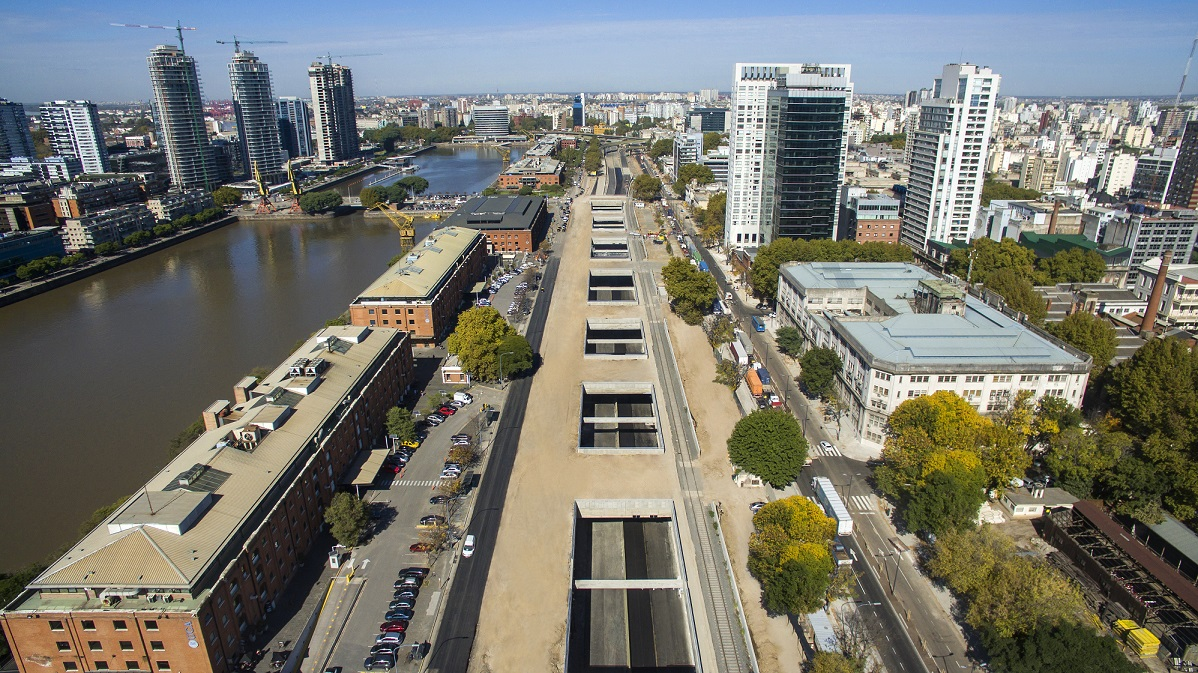
\includegraphics[width=0.80\textwidth]{images/Paseobajo.jpg}
    \caption{Paseo del bajo}
    \label{fig:}
\end{figure}
\end{frame}

\begin{frame}{Poniéndole precio a una carretera  II}
    \begin{figure} [H]
\centering
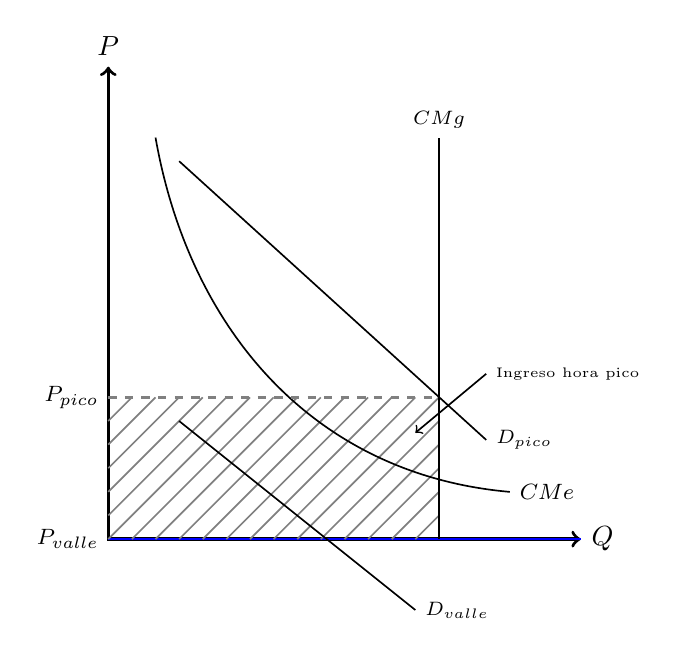
\begin{tikzpicture}[scale=0.6]
\draw[very thick,<->] (0,10) node[above]{$P$}--(0,0)--(10,0) node[right]{$Q$};
\draw[semithick, blue] (0,0)--(10,0);
\draw[semithick, gray] (0,2.5)--(0.5,3);
\draw[semithick, gray] (0,2)--(1,3);
\draw[semithick, gray] (0,1.5)--(1.5,3);
\draw[semithick, gray] (0,1)--(2,3);
\draw[semithick, gray] (0,0.5)--(2.5,3);
\draw[semithick, gray] (0,0)--(3,3);
\draw[semithick, gray] (0.5,0)--(3.5,3);
\draw[semithick, gray] (1,0)--(4,3);
\draw[semithick, gray] (1.5,0)--(4.5,3);
\draw[semithick, gray] (2,0)--(5,3);
\draw[semithick, gray] (2.5,0)--(5.5,3);
\draw[semithick, gray] (3,0)--(6,3);
\draw[semithick, gray] (3.5,0)--(6.5,3);
\draw[semithick, gray] (4,0)--(7,3);
\draw[semithick, gray] (4.5,0)--(7,2.5);
\draw[semithick, gray] (5,0)--(7,2);
\draw[semithick, gray] (5.5,0)--(7,1.5);
\draw[semithick, gray] (6,0)--(7,1);
\draw[semithick, gray] (6.5,0)--(7,0.5);
\draw [semithick] (1,8.5) to [out=280,in=175] (8.5,1)node [right] {\footnotesize $CMe$};
\draw [semithick] (7,0) to (7,8.5);
\node[above] at (7,8.5) {\scriptsize $CMg$};
\draw [semithick] (8,2.1) node [right]  {\scriptsize$D_{pico}$} to (1.5,8);
\draw [semithick] (6.5,-1.5) node [right]  {\scriptsize$D_{valle}$} to (1.5,2.5);
\draw[thick, gray, dashed](0,3)--(7,3) ;
\node[left] at (0,3){\footnotesize $P_{pico}$};
\node[left] at (0,0){\footnotesize $P_{valle}$};
\draw[semithick, ->] (8,3.5)--(6.5,2.25);
\node[right] at (8,3.5) {\tiny Ingreso hora pico};
\end{tikzpicture}
\label{fig:20.7}
\end{figure} 
 
\end{frame}


\begin{frame}{Externalidades}
    \begin{itemize}
        \item Sucede cuando una decisión económica genera un beneficio o costo no pecuniario
        \item Afecta a terceros que no son capaces de internalizar estos beneficios o costos
        \item La clave es que estos beneficios o costos ¡no se reflejan en los precios!
        \vspace{1mm}
        \item Dos tipos de externalidades: 
        \begin{itemize}
            \item Externalidades negativas: contaminación \vspace{1mm}
            \item Externalidades positivas: vacunación
        \end{itemize}
        
    \end{itemize}
\end{frame}

\begin{frame}{Un ejemplo}
    \begin{itemize}
        \item Dos productores: una curtiembre y pescadores
        \item La producción de curtiembres genera contaminación que afecta la cantidad de peces en el río
    \end{itemize}
\end{frame}

\begin{frame}{Curtiembres en Fez}

\begin{figure} [h!]
    \centering
    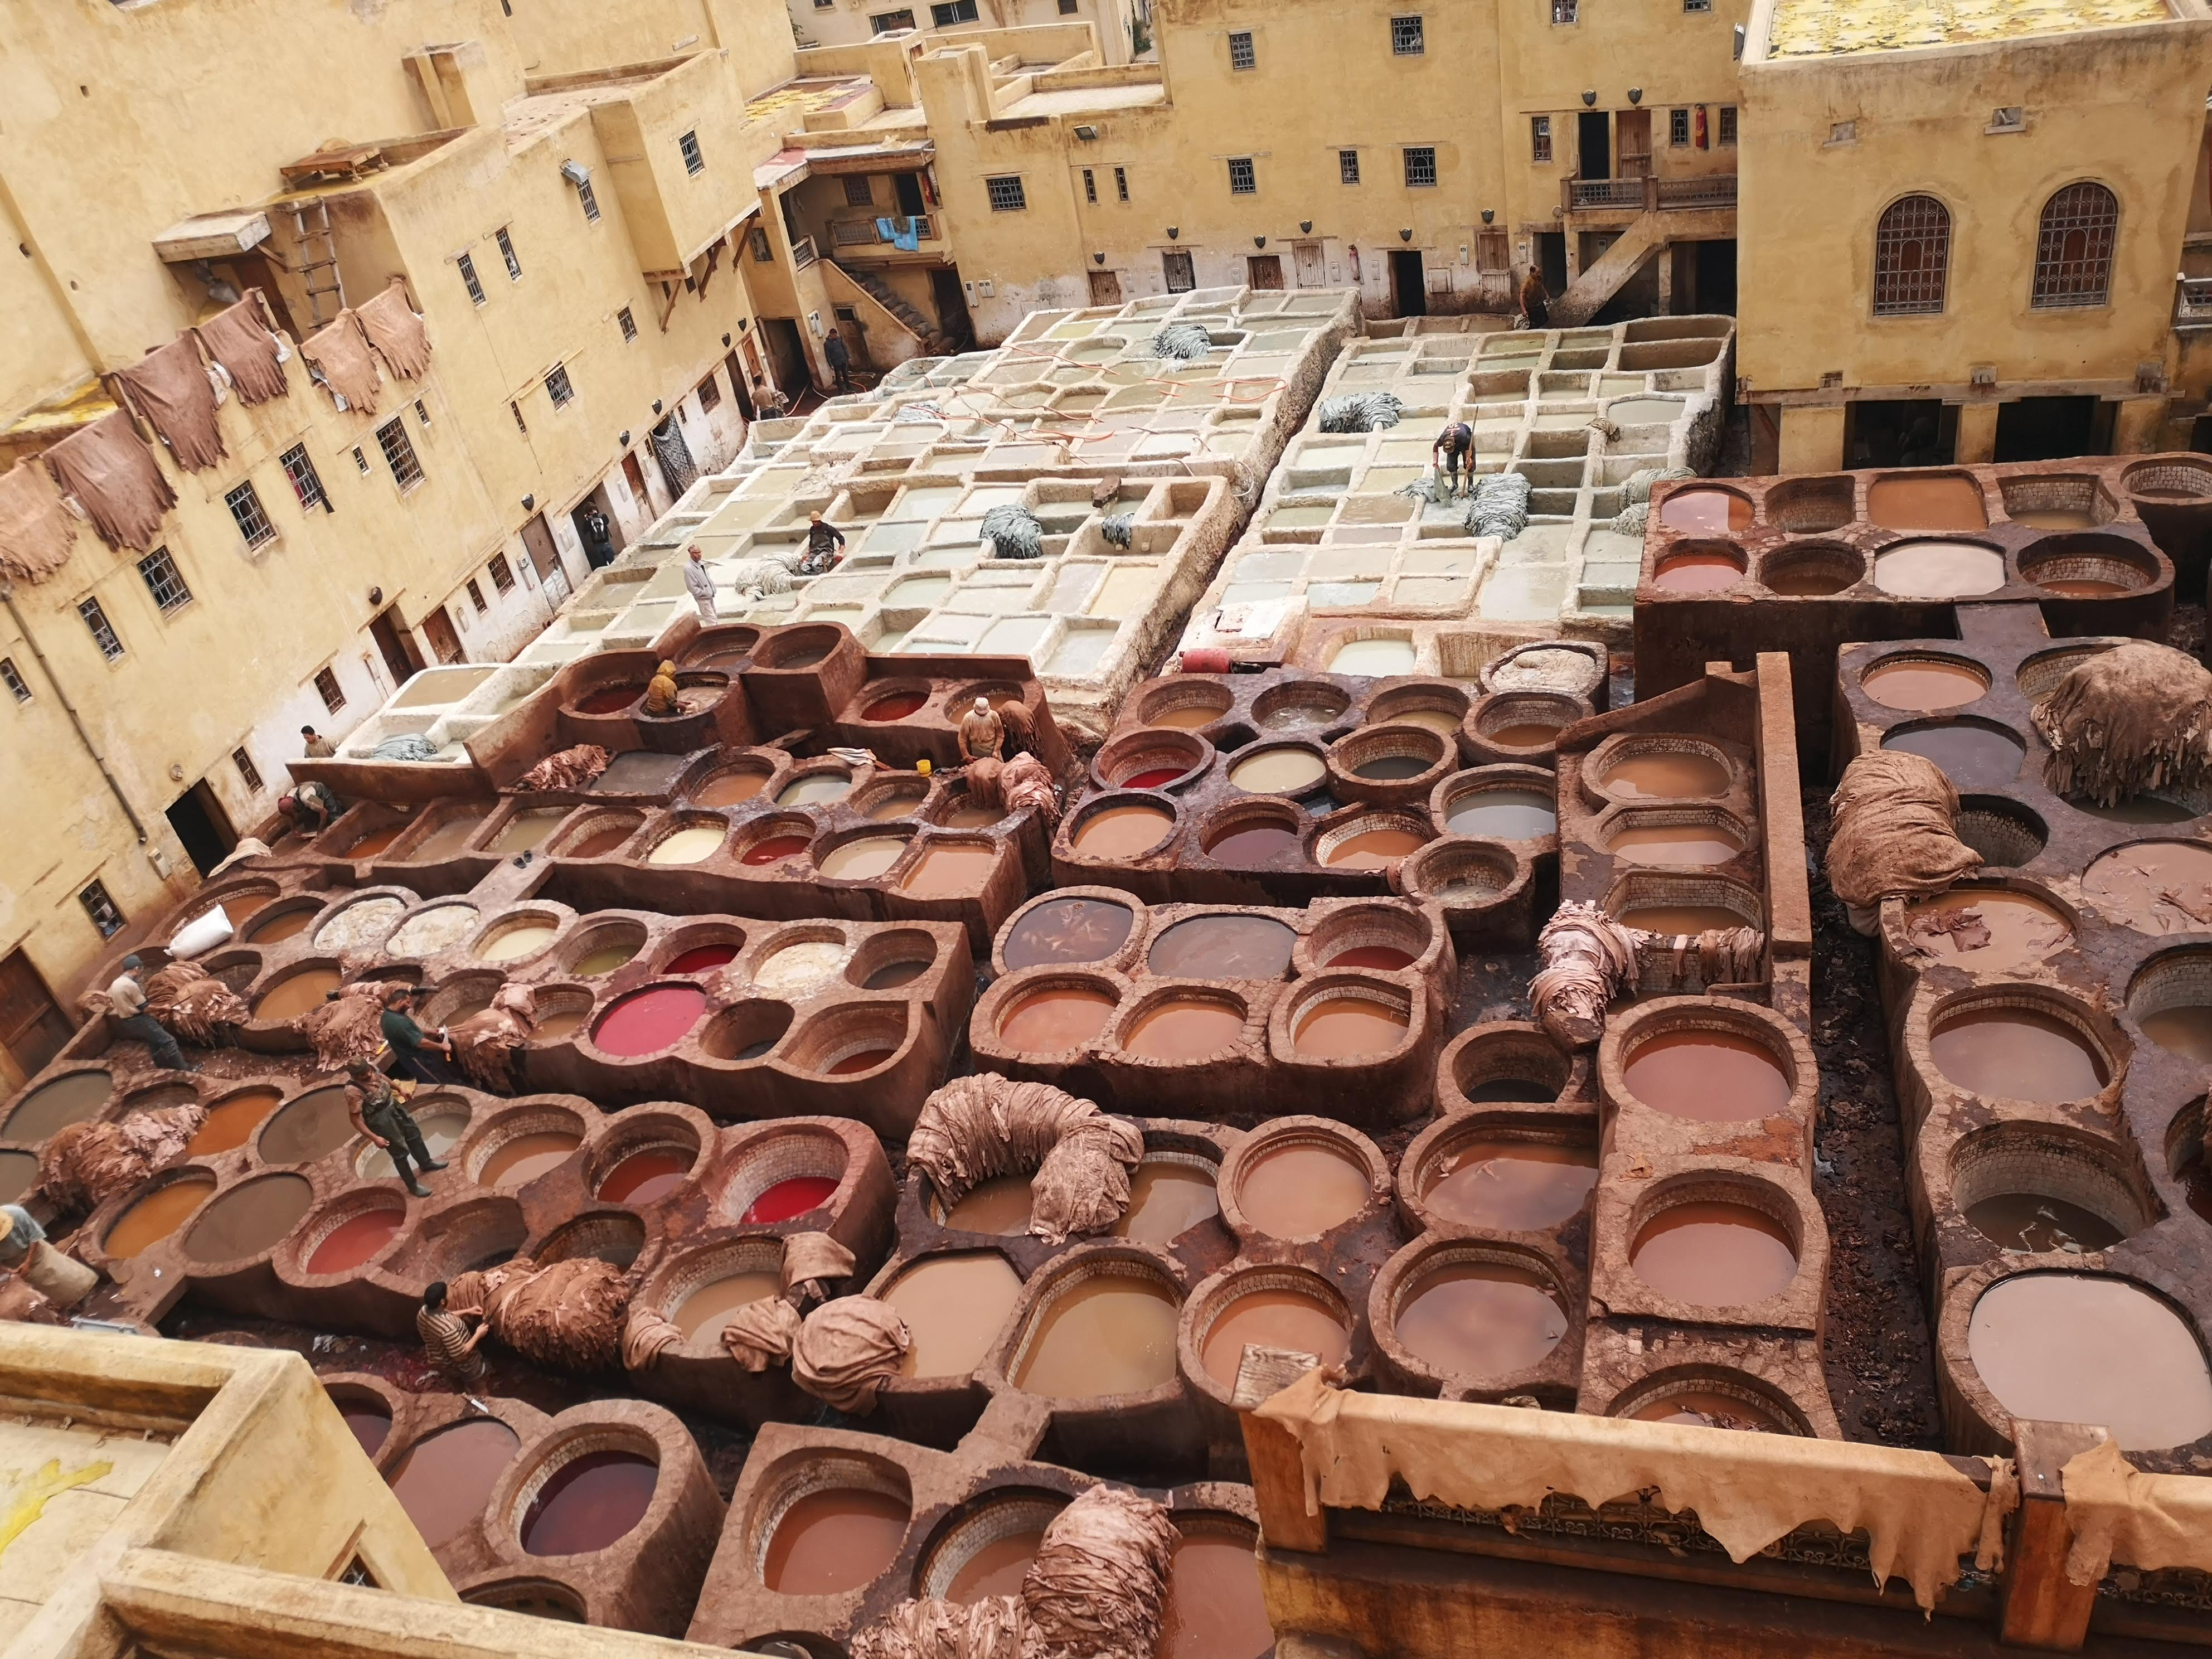
\includegraphics[width=0.8\textwidth]{Figures/Fez.jpg}
\end{figure}
\end{frame}

\begin{frame}{Como se suman los costos}
    \begin{figure} [H]
\centering
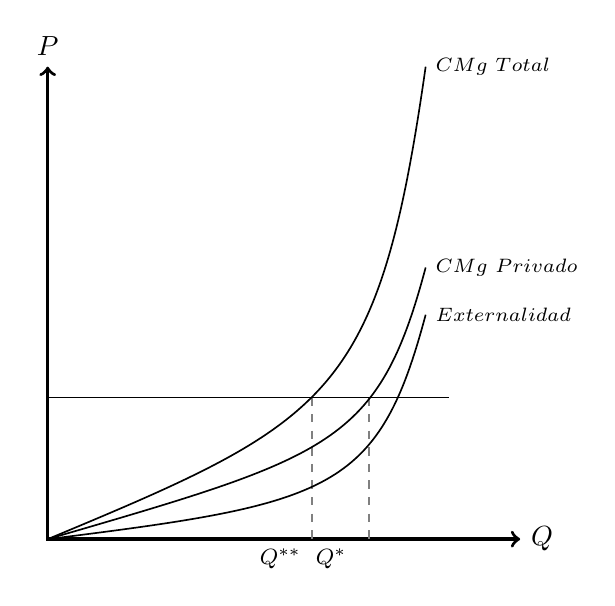
\begin{tikzpicture}[scale=0.6]
\draw[very thick,<->] (0,10) node[above]{$P$}--(0,0)--(10,0) node[right]{$Q$};
\draw[thick, dashed, gray] (5.6,3)--(5.6,0);
\draw[thick, dashed, gray] (6.8,3)--(6.8,0);
\draw [semithick] (0,0)..controls (6,1.75) and (7,2) .. (8,5.75) node [right] {\scriptsize $CMg \hspace{0.1cm} Privado$};
\draw [semithick] (0 ,0)..controls (6,0.75) and (7,1) .. (8,4.75) node [right] {\scriptsize $Externalidad$};
\draw [semithick] (0,0)..controls (6,2.5) and (7,3) .. (8,10) node [right] {\scriptsize $CMg \hspace{0.1cm} Total$};
\draw[semithick] (0,3)--(8.5,3);
\node[below] at (6,0) {\footnotesize $Q^{*}$};
\node[below] at (4.925,0) {\footnotesize $Q^{**}$};
\end{tikzpicture}
\end{figure} 
\end{frame}
 
\begin{frame}{Como corregir una externalidad}
    \begin{itemize}
        \item Regular la producción o el uso del contaminante
        \vspace{1mm}
        \item Gravar (con un impuesto) la actividad contaminante
    \end{itemize}
\end{frame}
  
\begin{frame}{Teorema de Coase}
    \begin{itemize}
        \item Coase dice que las externalidades no son un problema
        \item .... si los derechos de propiedad están bien definidos y los costos de transacción son nulos
        \item Esto es así porque ``hay una ganancia para apropiar'' de buscar un óptimo 
    \end{itemize}
\end{frame}

\begin{frame}{Coase I}
    \begin{figure} [H]
\centering
\begin{tikzpicture}[scale=0.6]
\draw[thick,<->] (0,10) node[above]{$P$}--(0,0)--(10,0) node[right]{$Q$};
\draw[fill,blue!15] (6.1,3.3)--(6.1,5)--(7.45,7.4)--(7.45,5)--(6.8,4);
%\draw[lines] (6.1,3.3)--(6.1,5)--(7.45,5)--(6.8,4);
%\draw[pattern=north west lines, pattern color=gray,solid] (6.1,3.3)--(6.1,5)--(7.45,5);
\path[pattern=horizontal lines,pattern color=black] (6.1,3.3)--(6.1,5)--(7.45,5);
\draw[thick, gray,dashed] (7.45,0)--(7.45,7.5);
\draw[thick, gray,dashed] (6.1,0)--(6.1,5);
\draw [semithick] (0,5) to (9,5) ;
\draw[semithick] (1,2)..controls (3,2) and (6,3) .. (8,9);
\draw[semithick] (1,1)..controls (3,1) and (7,2) .. (9,8.5);
\node[left] at (0,5) {\footnotesize $P^{*}$};
\node[below] at (7.45,0) {\footnotesize $Q^{*}$};
\node[below] at (6.1,0) {\footnotesize $Q^{**}$};
 \draw[semithick, <-] (6.75,4).. controls (7.15,3.75) and (7.7,3.75) ..(8.5,4);
\node [right] at (8.9,4.15) {\scriptsize Pérdida potencial};
\node [right] at (8.5,3.75) {\scriptsize Curtiembres};
\draw[semithick, <-] (6.85,5.8)--(5.75,7);
\node [right] at (3.75,7.75) {\scriptsize Pérdida Total};
\node [right] at (4.1,7.35) {\scriptsize Pescadores};

\end{tikzpicture}
\end{figure} 
\end{frame}
 
\begin{frame}{Coase II}
    \begin{figure} [H]
\centering
\begin{tikzpicture}[scale=0.6]
\draw[thick,<->] (0,10) node[above]{$P$}--(0,0)--(10,0) node[right]{$Q$};
\draw[fill,blue!15] (0.05,1.05)--(0.05,3)--(4.05,3)--(4.05,1.8)--(2,1.14)--(1,1.05);
\path[pattern=vertical lines,pattern color=black] (0,1)--(0,2)--(1.5,2)--(3,2.4)--(4.05,3)--(4.05,1.8)--(3,1.45)--(1.5,1.1);
\draw[thick, gray,dashed] (4.05,0)--(4.05,3);
\draw [semithick] (0,3) to (9,3) ;
\draw[semithick] (0.25,2)..controls (3,2) and (6,3) .. (8,9);
\draw[semithick] (0.25,1)..controls (3,1) and (7,2) .. (9,8.5);
\node[left] at (0,3) {\footnotesize $P^{*}$};
\node[below] at (4.05,0) {\footnotesize $Q^{**}$};
\draw[semithick, ->] (-0.5,1.5)--(0.5,1.5);
\draw[semithick, <-] (1.5,2.65)--(1.5,3.75);   
\node [right] at (0.5,4.5) {\scriptsize Ganancia };
   \node [right] at (0.25,4.1) {\scriptsize Curtiembres};
         \node [right] at (-3,1.75) {\scriptsize Pérdida };
   \node [right] at (-3.25,1.35) {\scriptsize Pescadores};
\end{tikzpicture}
\end{figure} 
\end{frame}

\begin{frame}{Bienes Públicos}
\begin{itemize}
    \item Vamos a distinguir los bienes por dos características
    \begin{itemize}
        \item Si su consumo es rival
        \item Si su consumo es excluible
    \end{itemize}
\end{itemize}
\end{frame}

\begin{frame}{Bienes Públicos}
\begin{table}[]
    \centering
    \begin{tabular}{|c|c|c|}
\hline
                      & \textbf{Rival}   & \textbf{No rival} \\ \hline
\textbf{Excluible}    & Bienes privados  & Bienes club       \\ \hline
\textbf{No Excluible} & Recursos comunes & Bienes públicos   \\ \hline
\end{tabular}
\end{table}
\end{frame}


\begin{frame}{Asimetrías de información}
    \begin{itemize}
        \item {\textbf{Riesgo moral o acción oculta}} alguien no puede ver las acciones del otro
            \begin{itemize}
            \item Ejemplos: seguros en general, incentivos a ahorrar, etc. 
            \end{itemize}
            \vspace{3mm}
        \item {\textbf{Selección adversa}} sucede cuando no conocemos una característica de la contraparte (atributos ocultos)
            \begin{itemize}
            \item Ejemplos: seguros en general, mercado de usados, empresas buscando contratar, etc.  
            \end{itemize}
            \end{itemize}
    \end{frame}

\begin{frame}{Ejemplos}
    \begin{itemize}
    \item \href{https://www.youtube.com/watch?v=qlg0qakJhKU}{\textbf{Matilda}}
    \item \href{https://www.youtube.com/watch?v=akA8co61He4}{\textbf{Tomates verdes fritos}}
    \item \href{https://www.youtube.com/watch?v=X8BPfLhH6MA}{\textbf{Friends}}
    \item \href{https://videos.criticalcommons.org/media/encoded/16/jtierney86/43ba1b1ac3e94df3974f987cc912ae_Hxgbfl1.mp4}{\textbf{The Daily Show}}
    \item \href{http://videos.criticalcommons.org/transcoded/http/www.criticalcommons.org/Members/JJWooten/clips/always-sunny-paying-for-care/video_file/mp4-high/always-sunny-cost-of-care-mp4.mp4}{\textbf{Always sunny}}
    \item \href{https://www.youtube.com/watch?v=SrPu-xGrKrk}{\textbf{Buying a car}}
    \item \href{https://www.youtube.com/watch?v=ZZq0ShjEd-E}{\textbf{But he has a Bud Light}}
    \end{itemize}

\end{frame}
    
\begin{frame}{El mercado de los limones de Akerlof}
\begin{itemize}
    \item Dos tipos de autos: buenos (q) y malos (1 - q)
    \begin{itemize}
    \item Para el vendedor el auto bueno vale 1000 y el lemon 500 
    \item Para el comprador el auto bueno vale 1500 y el lemon 750 
    \end{itemize} \vspace{3mm}
    \item Vamos a ver cuanto estaría dispuesto a pagar un comprador y dado eso después vemos que le conviene hacer al vendedor
    \begin{itemize}
    \item El comprador está dispuesto a pagar su valor esperado
    \end{itemize} \vspace{3mm}
    \item Si piensa que la probabilidad que un auto sea bueno sea  $\mu$ y que sea malo  $(1-\mu)$ el valor esperado para un auto típico en el mercado sería  $\mu 1500 + (1-\mu) 750= 750 + \mu 750$ 
\end{itemize}
\end{frame}

\begin{frame}{El mercado de los limones II}
\begin{itemize}
    \item El vendedor venderá un auto si lo que cobra por él supera su propia valoración:
    \vspace{3mm}
    \item Si tiene un auto malo lo venderá si 
    $500 \leq 750 + \mu 750$
    \begin{itemize}
    \item Esto se da siempre: quiere decir que si el vendedor tiene un lemon lo pone en el mercado siempre
    \end{itemize} \vspace{3mm}
    \item Si tiene un auto bueno, lo venderá si 
    $1000 \leq 750 + \mu 750 $ (1)
    \begin{itemize}
    \item Esto solo se daría si $\mu \geq \frac{1}{3}$
    \end{itemize} \vspace{3mm}
\end{itemize}
\end{frame}

\begin{frame}{El mercado de los limones III}
\begin{itemize}
    \item  Si $ q \geq \frac{1}{3}$, (hay suficiente buenos) hay un equilibrio donde $\mu = q \geq \frac{1}{3}$ y $p= 750 + \mu 750$ y se venden los dos tipos de autos 
    \vspace{1mm}
    \item Pero si $q \leq \frac{1}{3}$ entonces por la ecuación (1) sabemos que el auto no se vende
    \begin{itemize}
    \item El vendedor no tiene incentivos a tener autos nuevos, puesto que no los vendería en este caso
    \item Si $q= \mu = 0 $, quiere decir que se venden sólo limones y el precio de venta es de $p= 750$ 
    \end{itemize}
    \item El mercado para autos buenos desapareció aun cuando dijimos al principio que estos tenían más valor para los consumidores que para los vendedores \vspace{1mm}
    \item ¡La mano invisible de Adam Smith no pudo operar por la asimetría de información!
\end{itemize} 
\end{frame}

\begin{frame}{Riesgo moral y el colapso del mercado de seguros}
 \begin{itemize}
    \item Imaginemos una persona que tiene que comprar un seguro de incendio para su casa
    \begin{itemize}
    \item la casa puede no incendiarse y el individuo no pierde nada : Evento Bueno con probabilidad $p$
    \item la casa puede incendiarse y el individuo sufre una pérdida de tamaño $L$: Evento Malo con probabilidad $(1-p)$ 
    \end{itemize}
    \vspace{1mm}
    \item La probabilidad del evento bueno depende en parte de alguna acción del individuo, vamos a decir que depende del esfuerzo del individuo: $p(e)$
    \begin{itemize}
    \item Por ejemplo: el individuo esta alerta a no dejar electrodomésticos enchufados, ni hornallas encendidas, le hace mantenimiento al hagor, etc.
    \end{itemize}
    \item La clave es entender que quien ofrece el seguro no puede ver esta acción o esfuerzo
\end{itemize}
\end{frame}

\begin{frame}{Riesgo moral II}
    \begin{itemize}
    \item Si la compañía aseguradora ofrece una cobertura de valor $C$ a un precio $\pi C$ (el precio depende de la cobertura) \vspace{2mm}
    \item En el escenario bueno, la utilidad para el individuo es 
    $U_B = y - \pi C$
    \item Si se produce el evento malo, su utilidad para el individuo es 
    $U_M = y - L - \pi C + C$ \vspace{2mm}
    \item ¿Qué $\pi$ podría cobrar la compañía de seguros?
    \begin{itemize}
    \item La ecuación de ganancias de las aseguradoras es  
    $\pi C - (1-p) C$
    \item Si esta ganancia la hacemos $0$ el (menor) porcentaje que puede cobrar la compañía es $\pi=(1-p)$
    \end{itemize}
    \end{itemize}
\end{frame}

\begin{frame}{Riesgo moral III}
    \begin{itemize}
    \item Si el individuo compra una cobertura de $C=L$, es decir, se asegura totalmente:
    \begin{itemize}
    \item En el escenario bueno, la utilidad para el individuo es 
    $U_B = y - \pi L$
    \item Si se produce el evento malo, su utilidad para el individuo es 
    $U_M = y - L - \pi L + L = y - \pi L$ 
    \end{itemize}
    \item Le es indiferente si se produce el evento bueno o el malo 
    \item Pero entonces $e=0$, es decir, no va a esforzarse por cuidar la casa, y la probabilidad del evento malo va a ser más alta \vspace{2mm}
    \item Si el individuo no hace nada el siniestro ocurre con probabilidad $(1-p)=1$, y en este caso, $p=0$ y $\pi=1$
    \item La utilidad para el individuo de comprar seguro es $y-L$, que resulta peor que no comprar seguro $y$
    \item ¡Es decir que el mercado asegurador desaparece! 
  \end{itemize}   
\end{frame}


\begin{frame}{Discusiones}
    \begin{itemize}
        \item ¿Por qué pierden valor los autos al salir de la concesionaria? \vspace{1mm}
        \item Políticas de deducibles \vspace{1mm}
        \item Obama care
    \end{itemize}
\end{frame}


\end{document}